\section{Scheduling with Unknown Output Lengths: The Nested WAIT Algorithm}
\label{sec:nested_wait}

The WAIT algorithm assumes that output lengths are known when thresholds are set. Nested WAIT relaxes this requirement by using output-length information only as it is revealed by the prompt's own decode trajectory. The \textit{Nested Waiting for Accumulated Inference Threshold} (Nested WAIT) algorithm organizes decoding into nested segments and controls how prompts advance across those segments. In this setting, endogenous memory growth is harder to control because the scheduler does not know, at admission, which resident prompts will continue into later decode stages. Nested WAIT reduces this unknown-output-length state to segment-boundary queues that track the surviving prompts most likely to create downstream memory pressure.

\subsection{Algorithm Overview}

We first return to the running example to show how unknown output lengths complicate policy design and memory control. The same admitted prompts may either finish at an early decode boundary or continue to later decode stages with larger KV caches, so neither an optimistic nor a conservative admission rule is satisfactory.

\begin{example}[Unknown Output Lengths]
\label{ex:unknown_output}
Continuing Example~\ref{ex:fcfs_cascade}, suppose output lengths are now \emph{unknown} at arrival: each ``Hello'' prompt receives either ``Hi'' (1 token) or ``Hi there!'' (2 tokens). The scheduler faces a dilemma. If it optimistically treats all outputs as short, then capacity \(C=12\) appears to allow 6 prompts, because each would use 2 units after one decode token. If some prompts instead generate two tokens and require 3 units each, the same admission decision can overflow memory and trigger eviction. A conservative rule that treats every prompt as long avoids this overflow, but admits only 4 prompts and wastes capacity whenever most prompts are short.
\end{example}

Nested WAIT avoids both extremes by pooling prompts in early decode stages and separating them only at completion boundaries. Segment 1 serves all prompts until the first possible output length \(l_1'\); prompts that complete there leave the system and release memory, while the remaining prompts enter Segment 2. The same logic repeats across later boundaries. The policy therefore does not reserve memory for long outputs before they are observed, but still lets short prompts complete without waiting behind longer ones.

Formally, let output lengths satisfy $l_1' < l_2' < \dots < l_m'$, where type $j$ has decode length $l_j'$, and set $l_0'=0$. Nested WAIT defines \(m\) segments, with segment \(k\) covering the decode work between boundaries \(l_{k-1}'\) and \(l_k'\). The segment receives types \(k,k+1,\dots,m\), whose combined arrival rate is \(\lambda_k+\cdots+\lambda_m\). The threshold vector \(\pi=[n_1,\dots,n_m]\) has two roles: \(n_k\) caps the number of prompts processed per prefill/decode stage in segment \(k\), and it is also the number of prompts that must be available at the segment's entry boundary before that segment begins service.

The hidden output-length labels are i.i.d. across prompts according to the arrival mix, and Nested WAIT is nonanticipating: before a prompt reaches a segment boundary, the scheduler does not use whether that prompt will complete there or continue downstream.

Thus, if segment \(k^*\) has fewer than \(n_{k^*}\) prompts at its entry boundary, Nested WAIT pauses segment \(k^*\) and all later segments while retaining their KV caches on the GPU. This is a scheduling preemption, not a memory swap: resident prompts waiting at a downstream boundary or inside a segment continue to count against GPU memory. Only prompts still outside the GPU before prefill, namely the external entry queue of Segment 1, have no resident KV cache. Earlier segments \(k<k^*\) can continue batching up to \(n_k\) prompts per prefill/decode stage, so new arrivals can keep moving through the shared early segment. Once enough prompts reach the boundary of segment \(k^*\), that segment resumes. Algorithm~\ref{alg:nested_wait} formalizes this procedure, and Figure~\ref{fig:nested_wait} illustrates the resulting pipeline.

Nested WAIT's segmentation rule is based on decode progress. For the main analysis, we take a common prefill length \(l\) to keep the memory expressions transparent; Appendix~\ref{sec:extension} discusses heterogeneous prefill lengths and coarser segmentations.
% We leave the discussion in Appendix \ref{sec:extension}.

\begin{figure}[h]
    \centering
    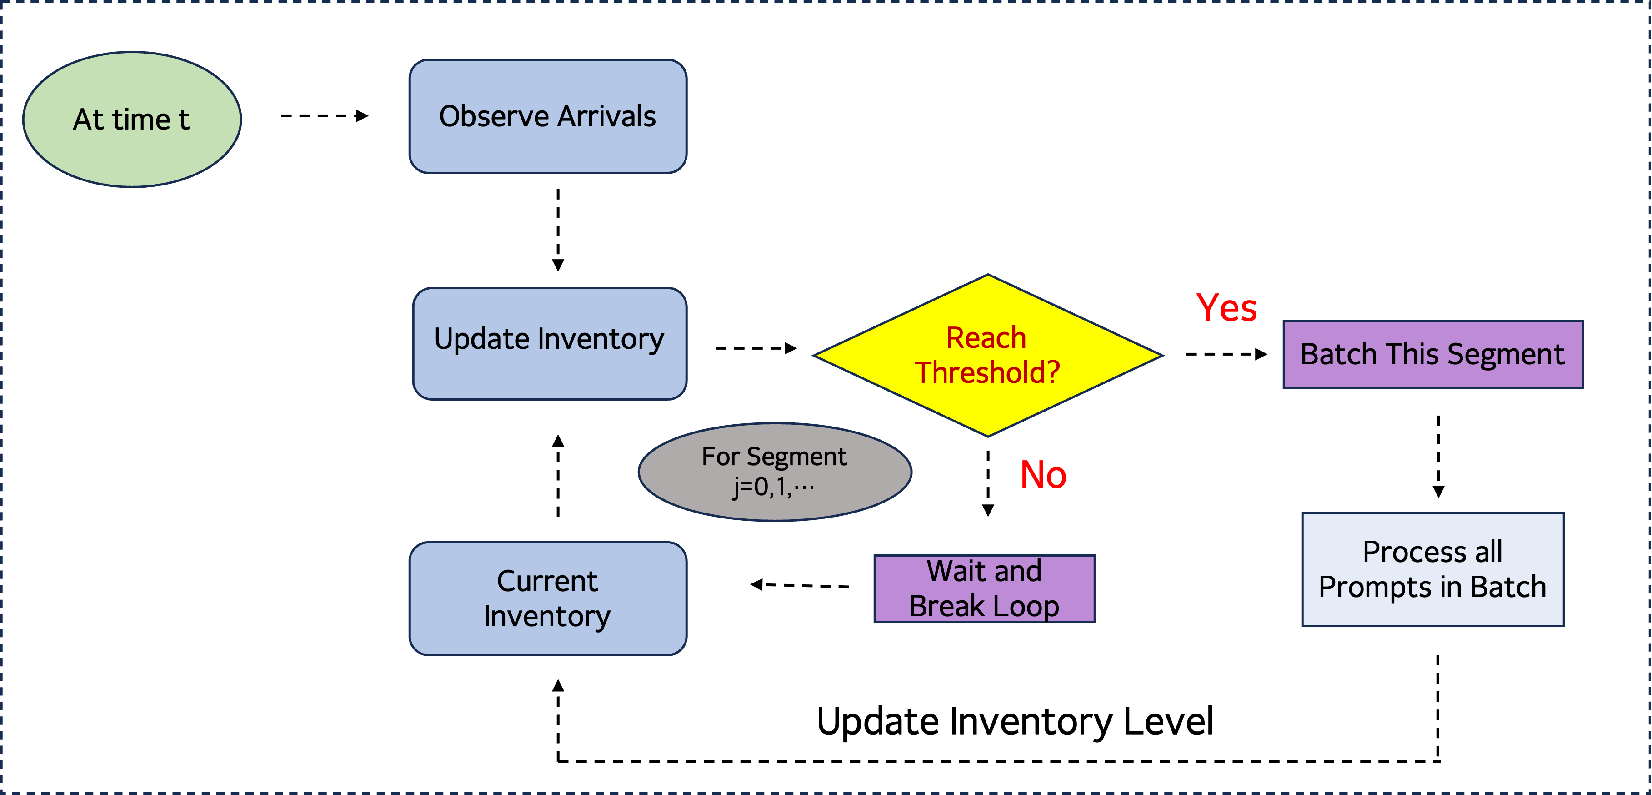
\includegraphics[width=0.85\linewidth]{Experiments_pdf/fig_nestedWAIT.pdf}
    \caption{Nested WAIT pipeline. Prompts enter the first segment without output-length labels; short prompts complete and exit at early boundaries, while longer prompts advance to later segments where separate thresholds regulate batching.}
    \label{fig:nested_wait}
\end{figure}
In the two-type instance from Example~\ref{ex:unknown_output}, Nested WAIT uses two segments. Segment 1 processes all newly arrived prompts through prefill/decode stages \(0\) and \(1\) at combined rate \(\lambda_1+\lambda_2\); type-1 prompts then complete, while type-2 prompts enter Segment 2 and are processed at rate \(\lambda_2\). Figure~\ref{fig:nested_wait_example} shows this operation over time. Segment 1 waits until enough newly arrived prompts have accumulated, and Segment 2 waits until enough prompts have survived the first segment. When both thresholds are met, the active segments are scheduled together. Thus early segments provide shared batching, while later segments regulate service for prompts that have been identified as longer jobs.


\begin{figure}[h]
    \centering
    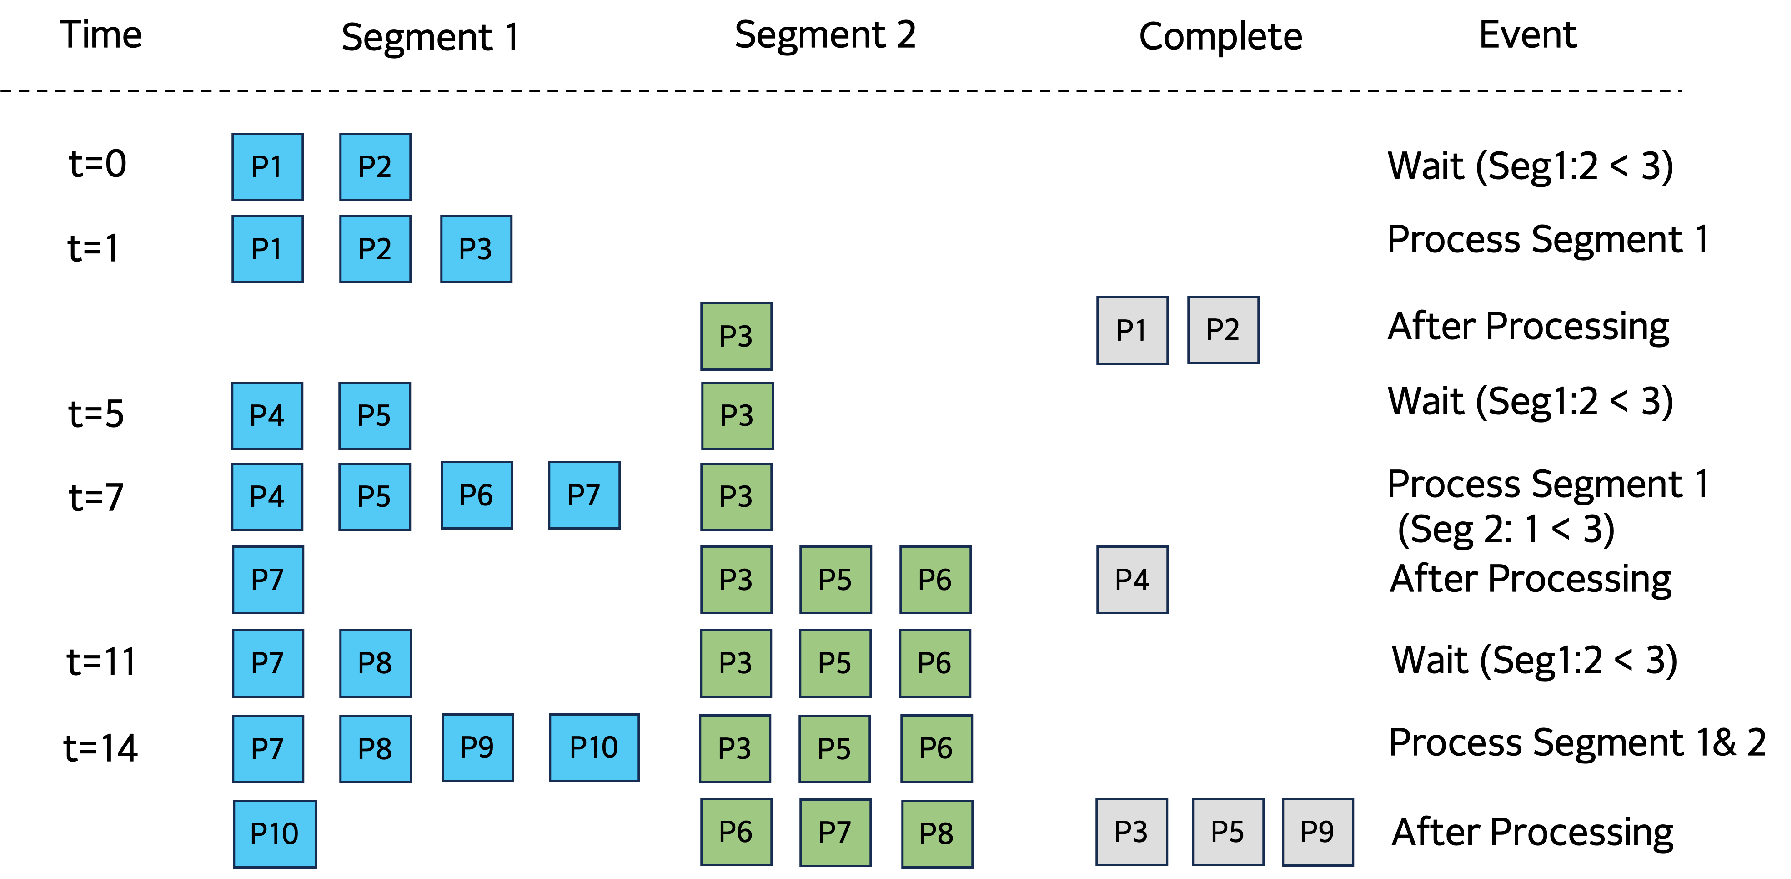
\includegraphics[width=0.85\linewidth]{Experiments_pdf/fig_nestedWAIT_example.pdf}
    \caption{Two-segment Nested WAIT example. Segment 1 batches newly arrived prompts once its threshold is met; Segment 2 starts only after enough prompts have survived the first segment and revealed themselves as longer jobs.}
    \label{fig:nested_wait_example}
\end{figure}

\begin{algorithm}[h]
\caption{Nested WAIT: Nested Waiting for Accumulated Inference Threshold}
\label{alg:nested_wait}
{\small\linespread{1.0}\selectfont
\begin{algorithmic}[1]
\Require Memory capacity \( C \), arrival rates \( \lambda_j \) for \( j \in [m] \), thresholds \( n_k \) for segments \( k \in [m] \)
\Require Output lengths \( l_1' < l_2' < \cdots < l_m' \) for output-length classes \( j \in [m] \)
    \Statex \Comment{$Q_{1,0}$ is the external prefill queue; for $k\ge2$, $Q_{k,l_{k-1}'}$ is the resident boundary queue}
    \Statex \Comment{The threshold-controlled interior of segment $k\ge2$ consists of stages $l_{k-1}'+1,\ldots,l_k'$}
    \State Initialize all segment-entry, boundary, and interior queues to zero
\State Initialize event queue; set current time \( t \gets 0 \)
\State Set server status to idle
\While{True}
    \State Wait for the next event (arrival or batch completion)
    \If{event is an arrival}
        \State \( Q_{1,0} \gets Q_{1,0} + 1 \)  \Comment{New prompts enter segment 1 at stage 0}
    \ElsIf{event is a batch completion for prefix \(1,\dots,k\)}
        \State Retrieve the selected counts \(a_{k's}\) stored with the completed prefix batch
        \State Update all affected queues simultaneously using the stored selected counts
        \For{each processed segment \( k'\le k \)}
        \For{each selected stage \(s\) with stored count \(a_{k's}\)}
            \If{\(k'\ge2\) and \(s=l_{k'-1}'\)}
                \State Move selected boundary prompts to the first interior stage \(l_{k'-1}'+1\)
            \ElsIf{\(s<l_{k'}'\)}
                \State Move selected interior prompts to stage \(s+1\)
            \Else
                \If{\(k'<m\)}
                    \State Complete prompts whose output ends at \(l_{k'}'\); move survivors to \(Q_{k'+1,l_{k'}'}\)
                \Else
                    \State Complete and clear KV caches
                \EndIf
            \EndIf
        \EndFor
        \EndFor
        \State Set server status to idle
    \EndIf
    \State Find largest \( k \) such that \( Q_{k', l_{k'-1}'} \geq n_{k'} \) for all \( k' \leq k \) \Comment{All segments up to $k$ meet threshold}
    \If{server is idle and such \( k \) exists}
        \State Set \(S_1=\{0,\ldots,l_1'\}\)
        \State For \(k'=2,\ldots,k\), set \(S_{k'}=\{l_{k'-1}',\ldots,l_{k'}'\}\)
        \State For every \(k'\le k\) and \(s\in S_{k'}\), set \(a_{k's}\gets\min\{n_{k'},Q_{k',s}\}\)
        \State Form the prefix batch from all selected prompts and store \(a_{k's}\)
        \State Process batch; already resident prompts outside the batch wait with their KV caches retained
        \State Set server status to busy until the completion event for this prefix batch
    \EndIf
\EndWhile
\end{algorithmic}
}
\end{algorithm}

Algorithm~\ref{alg:nested_wait} gives the formal description of Nested WAIT. Completion events determine which prompts exit and which continue downstream; thresholds determine when each active segment has enough work to process without sacrificing batching efficiency.

\subsection{Main Theorem}
\label{subsec:nested_main_theorem}

The analysis uses the same asymptotic scaling and scaled delay metrics as Section~\ref{sec:wait}: arrivals and service speed scale with \(\zeta\), and the effective horizon in the bounds is \(\zeta T\). As in WAIT, \(M^\pi\) denotes the base threshold memory and is independent of \(\zeta\). The required physical memory \(M_{\mathrm{req}}^{(\zeta,\pi)}\), however, also includes the logarithmic safety buffer in \eqref{eq:nested_wait_memory_total}; this buffer is the finite-horizon cost of controlling downstream boundary queues. Equivalently, for a fixed physical memory capacity, the theorem applies to horizons and failure probabilities for which \(C\ge M_{\mathrm{req}}^{(\zeta,\pi)}\). The new difficulty is that downstream segments receive endogenous input. The prompts entering segment \(k\) are exactly those that survived earlier segments, so their arrivals depend on upstream batching, completion events, and the resident KV caches carried across segment boundaries. We study throughput \(\throughput^{(\zeta,\pi)}\), latency \(\Latency^{(\zeta,\pi)}\), and time to first token \(\TTFT^{(\zeta,\pi)}\) under a threshold vector \(\pi=[n_1,\dots,n_m]\).

The need for additional memory is already visible at \(C=M^*\). At this capacity, the fluid equilibrium fits in memory if output lengths are known. A non-predictive policy, however, must admit prompts before knowing whether they will finish at an early boundary or continue downstream. Optimistic admission can overflow memory once prompts reveal longer outputs; conservative admission avoids that risk but leaves capacity unused. The resulting uncertainty creates a non-vanishing throughput loss.

\begin{proposition}
\label{prop:unknown_lower_bound}
When memory capacity is exactly at the fluid stability boundary, \(C=M^*\), there exists an instance where any online non-predictive policy \( \pi \), unaware of output lengths upon arrival, incurs a throughput gap \( \throughput^* - \mathbb{E}[\throughput^{(\zeta, \pi)}] = \Omega(1) \).
\end{proposition}

This lower bound shows that uncertainty has a memory cost: \(M^*\) supports the fluid equilibrium with known output lengths, but does not provide enough room for the boundary queues created by unknown output lengths. The proof constructs a two-output-length instance in which the number of prompts continuing past the first boundary has binomial fluctuations (Appendix~\ref{appendix:proof_unknown_lower_bound}). Theorem~\ref{thm:nested_wait_heavy_traffic} shows that Nested WAIT closes this gap with a logarithmic safety buffer. The construction has two parts: choose thresholds that give these boundary queues negative drift, and reserve enough memory for their residual stochastic fluctuations.

The threshold vector must make each segment queue stable while keeping batches large enough to exploit the GPU. Let \(\Delta T_{[1,\dots,m]}(n_1,\dots,n_m)\) denote the iteration time when segment \(k\) contains exactly \(n_k\) prompts at each prefill/decode stage in that segment. The required drift conditions are
\begin{equation}
    \label{eq:nested_wait_thresholds}
    \begin{aligned}
    &\Delta T_{[1,\dots,m]}(n_1, \dots, n_m) <\frac{n_1}{\sum_{j=1}^m \lambda_j}, \\
    &p_k < \frac{n_k}{n_{k-1}} < 1,\quad \forall k \in \{2, \dots, m\},
    \end{aligned}
\end{equation}
where \(p_k = (\sum_{j=k}^m\lambda_j)/(\sum_{j=k-1}^m\lambda_j)<1\) for \(k\ge2\). The first inequality gives negative drift for the entry queue of Segment 1. The second gives negative drift for each downstream boundary queue, since only a \(p_k\) fraction of prompts leaving segment \(k-1\) continue to segment \(k\); the upper bound \(n_k<n_{k-1}\) keeps the boundary queue in the nondegenerate binomial-tail regime used in the martingale-root bound. If \(n_k\ge n_{k-1}\), the downstream boundary queue is deterministically bounded and can be handled separately without this logarithmic tail term. Segments with \(p_k=0\) have no stochastic downstream input and can be omitted or merged. For memory accounting, define
\[
\delta_1=l_1'+1,\quad \bar s_1=\frac{l_1'}{2},\qquad
\delta_k=l_k'-l_{k-1}',\quad \bar s_k=\frac{l_{k-1}'+1+l_k'}{2}\quad (k\ge2).
\]
The base memory used by threshold-sized segment batches is
\begin{equation}
    \label{eq:nested_wait_memory}
\begin{aligned}
        M^\pi &= \sum_{k=1}^m n_k (l+\bar s_k)\delta_k .
\end{aligned}
\end{equation}
Here \(\delta_k\) is the number of prefill/decode stages covered by segment \(k\), and \(\bar s_k\) is the average decode progress across those stages. The term \(M^\pi\) is the threshold analogue of the fluid memory requirement \(M^*\): if \(n_k\) is chosen on the scale of the cumulative fluid population that survives to segment \(k\), then \(M^\pi\) is on the same scale as \(M^*\), up to rounding and segment aggregation.

For \(k\ge2\), the resident queue at boundary \(l_{k-1}'\) is measured after the threshold review for segment \(k\). When segment \(k\) is selected, the \(n_k\) boundary prompts removed from this queue are charged to the first interior stage of segment \(k\) in \(M^\pi\), which is a safe upper bound because that stage has one additional decode token. The additional memory buffer in the theorem counts only boundary prompts not selected in the current prefix batch. Appendix~\ref{sec:segment_design}, especially Figures~\ref{fig:fixed_T_200_rate_50_delta_0.1_1e-5}--\ref{fig:fixed_delta_0.001_rate_50_T_20_2000}, gives a numerical decomposition showing this base term relative to the safety buffers. With these definitions, the theorem below gives the performance guarantee.

Thus \(M^*\le C\) is the fluid-model stabilizability condition when output lengths are known. With unknown output lengths, Nested WAIT also needs enough memory for the downstream boundary queues created as prompts reveal whether they continue to later segments. The theorem below shows that, with this additional safety buffer, Nested WAIT realizes the corresponding stability guarantee in the stochastic system.

\begin{theorem}
\label{thm:nested_wait_heavy_traffic}
Assume thresholds \( \pi = [n_1, \dots, n_m] \) satisfy \eqref{eq:nested_wait_thresholds}, and the physical memory capacity \(C\) satisfies
\begin{equation}
    \label{eq:nested_wait_memory_total}
\begin{aligned}
    C &\ge M_{\mathrm{req}}^{(\zeta,\pi)}
:= M^\pi + \sum_{k=2}^m (l + l_{k-1}') \bigg(n_k + \theta_k^{-1} \ln\Big( \frac{m(1+\zeta T/d_0)}{\delta} \Big)\bigg) \\
&= O\bigg( M^\pi + \sum_{k=2}^m (l + l_{k-1}') \theta_k^{-1}\ln\Big( \frac{m(1+\zeta T/d_0)}{\delta} \Big) \bigg),
\end{aligned}
\end{equation}
where $\theta_k>0$ is the unique solution of \(e^{-\theta_k n_k}(1-p_k+p_ke^{\theta_k})^{n_{k-1}}=1\); in particular, $\theta_k \geq 8(n_k - n_{k-1}p_k)/n_{k-1}$ for \(k\ge 2\). For the corresponding no-overflow Nested WAIT dynamics:
$$
    \begin{aligned}
        &\throughput^* - \mathbb{E}\big[ \throughput^{(\zeta, \pi)} \big] 
   = O\big( (\zeta T)^{-1} \big), \\
&\mathbb{E}\big[ \Latency^{(\zeta, \pi)} \big],\,\mathbb{E}\big[ \TTFT^{(\zeta, \pi)} \big] = O(1).
    \end{aligned}
$$
Moreover, the no-overflow dynamics are feasible on the physical GPU, i.e., memory is not exceeded, with probability at least \(1-\delta\) over horizon \([0,T]\).
\end{theorem}

Unknown output lengths make this memory-control problem harder. At admission, the scheduler does not know which prompts will finish early and which will continue into later, more memory-intensive decode stages. Yet endogenous memory growth starts as soon as a prompt's KV cache becomes resident on the GPU. As Example~\ref{ex:unknown_output} illustrates, prompts reveal their output lengths only by either completing at a boundary or continuing beyond it. Completed prompts leave and release memory, while surviving prompts carry larger KV caches downstream. Without segment-level control, these surviving prompts can create late-stage buildup, overflow memory, and trigger eviction-induced restarts. Nested WAIT therefore regulates both admission and advancement through prefill and decode while the output-length mix is still being revealed.

The proof follows the prompts at these segment boundaries, where output-length information is revealed and downstream memory growth must be controlled. Conditional on a threshold-sized batch leaving segment \(k-1\), the number that continue to segment \(k\) follows binomial thinning with probability \(p_k\). This coupling turns the unknown-output-length process into boundary queues. These queues track how much surviving work is allowed to continue into later segments, which is the part of the memory-growth trace that can cause overflow. In the memory condition \eqref{eq:nested_wait_memory_total}, \(M^\pi\) covers threshold-sized segment batches, while the remaining terms keep retained KV caches at downstream boundaries from causing overflow and eviction. The theorem states the clean case with one boundary per output length. In practice, the number of possible output lengths can be large, and the same construction can be implemented with coarser decode segments that group nearby lengths and maintain thresholds only at the segment boundaries. Appendix~\ref{sec:extension} discusses this general segment design, and Section~\ref{sec:experiments} evaluates it in simulated serving workloads.
